\documentclass[xcolor=pdftex,dvipsnames,table,aspectratio=169]{beamer}
%\documentclass[xcolor=pdftex,dvipsnames,table,handout,aspectratio=169]{beamer}

%\setbeameroption{show notes}

\usepackage{bm,graphicx,multirow,amsmath,tikz} %fancybox,
\usepackage{color}%,textpos}
\usepackage[round]{natbib}
\usepackage[normalem]{ulem}
\usepackage{hyperref}
\usepackage{lastpage}
\usepackage{array}
\usepackage{color}
\usepackage{framed}
\usepackage{hyperref}

% Define Western colours
\definecolor{western}{rgb}{.306,.152,.524}
\definecolor{westerngray}{rgb}{.512,.508,.524}

%% Define BEAMER colours
\setbeamercolor{frametitle}{bg=western,fg=white}
\setbeamercolor{framesubtitle}{bg=western,fg=black}
\setbeamercolor{title}{fg=white,bg=western}
\setbeamercolor{author}{fg=white,bg=western}
\setbeamercolor{institute}{fg=white,bg=western}
\setbeamercolor{date}{fg=white,bg=western}

%% Set BEAMER fonts
\setbeamerfont{title}{shape=\bf}
\setbeamerfont{frametitle}{shape=\sc,size=\Large}
\setbeamerfont{framesubtitle}{shape=\sc,size=\Large}
\setbeamerfont{footline}{shape=\sc}

%% Define BEAMER toc
\setbeamercolor{section in toc}{fg=western}
\setbeamercolor{subsection in toc}{fg=westerngray}
\setbeamertemplate{sections/subsections in toc}[ball]

%% Define BEAMER background
\setbeamercolor{background canvas}{bg=white}

%% Define BEAMER footer
\setbeamertemplate{navigation symbols}{}
\setbeamercolor{footline}{fg=white,bg=western}
\setbeamertemplate{footline}{%
  \begin{beamercolorbox}[wd=\paperwidth]{footline}
    \vskip5pt

    \raisebox{.05in}{
      \scriptsize{\bf \insertshorttitle}
    }
    \hfill
    \raisebox{.05in}{
      \scriptsize{\bf \insertframenumber/\inserttotalframenumber} 
    }
    \hspace{5pt}

    \vskip5pt
  \end{beamercolorbox}
}

%% Define BLOCK environment
\setbeamercolor{block title}{fg=western}
\setbeamerfont{block title}{series=\bfseries}

%% Define ENUMERATE and ITEMIZE environements
\setbeamertemplate{itemize item}[ball]
\setbeamertemplate{enumerate item}[ball]
\setbeamercolor{item projected}{bg=western}

%% Define BEAMER toc
\setbeamercolor{sections/subsections in toc}{fg=blue!75}
\setbeamertemplate{sections/subsections in toc}[ball]

% %% Define SECTION openings
% \AtBeginSection[]{
%   \begin{frame}{\insertshorttitle}
%     \tableofcontents[currentsection,subsectionstyle=hide/hide/hide]
    
%   \end{frame}
% }

%% Define BEAMER frametitle
\addtobeamertemplate{frametitle}{
   \let\insertframetitle\insertsectionhead}{}
\addtobeamertemplate{frametitle}{
   \let\insertframesubtitle\insertsubsectionhead}{}


\makeatletter
  \CheckCommand*\beamer@checkframetitle{\@ifnextchar\bgroup\beamer@inlineframetitle{}}
  \renewcommand*\beamer@checkframetitle{\global\let\beamer@frametitle\relax\@ifnextchar\bgroup\beamer@inlineframetitle{}}
\makeatother

% Define counters for example and exercise
\newcounter{example}
\newcounter{exercise}

% Define example and exercise commands
\renewcommand{\example}
{\stepcounter{example}Example \lecturenum.\arabic{example}}
\newcommand{\examplectd}
{Example \lecturenum.\arabic{example}\ ctd}
\newcommand{\exercise}
{\stepcounter{exercise}Exercise \lecturenum.\arabic{exercise}}
\newcommand{\exercisectd}
{Exercise \lecturenum.\arabic{exercise}\ ctd}

\newcommand{\lecturenum}{14}

\title[SS2857]{Probability and Statistics I}
\subtitle{\lecturenum. Continuous Random Variables and Probability Distributions}

\date{Revised 31/10/24}

%% Add logo
% \titlegraphic{\includegraphics[height=2cm]{../uwo_logo_reversed}}

%% Initialize R


\begin{document}

{
\setbeamertemplate{footline}{}
\setbeamercolor{background canvas}{bg=western}

\begin{frame}
  \addtocounter{framenumber}{-1}

  \maketitle
\end{frame}
}

\section{Discrete Random Variables}

%\begin{frame}
%
%  \begin{block}{Review Exercise}
%    Suppose that you are in downtown London on a cold, rainy night in October and you want to take a taxi home. Taxis pass the point where you are at an average rate of 1 per 5 minutes and 9 out of every 10 taxis are already full.

%    \bigskip

%    Identify the distributions of the following random variables. Be as specific as you can.

%    \bigskip

%    \begin{enumerate}
%    \item The number of taxis that pass the point where you are in 20 minutes.
%    \item The number of taxis that pass until the first empty taxi arrives.
%    \item The number of empty taxis within the first 15 taxis that pass.
%    \end{enumerate}
%  \end{block}
  
%\end{frame}

\section{Continuous Random Variables}

\begin{frame}
  \frametitle{\invisible{Hello}}

  \begin{center}
    \Large{\textbf{4.1 Continuous Random Variables}}
  \end{center}

  % \begin{center}
  %   
\includegraphics[height=.5\textheight]{roulette_wheel}
  % \end{center}

\end{frame}

\begin{frame}

  \begin{block}{Probability Density Functions}
    Let $X$ be a continuous random variable. Then the probability density function (pdf) of $X$ is a function $f(x)$ such that for any two numbers $a$ and $b$ with $a \leq b$,
    \[
      P(a \leq X \leq b)=\int_a^b f(x)~dx.
    \]

    \bigskip

    For $f(x)$ must satisfy two properties to be a valid pdf:
    \begin{enumerate}
    \item $f(x) \geq 0$ for all $x \in \mathbb{R}$
    \item $\int_{-\infty}^\infty f(x)~dx = 1$
    \end{enumerate}
    
  \end{block}
\end{frame}


\begin{frame}

  \begin{block}{Cumulative Distribution Function}
    The cumulative distribution function $F(x)$ for a continuous random variable with pdf $f(x)$ is defined as
    \[
      F(x)=P(X \leq x)=\int_{-\infty}^x f(y)~dy.
    \]
    for every $x \in \mathbb R$.

    \bigskip

    Alternatively, if $X$ is a continuous random variable with cdf $F(x)$ then \textit{one possible}\footnote{The proposition on page 166 of the textbook is not entirely accurate. Differentiating the cdf provides one possible pdf, but the pdf is not unique. The details are beyond this course, but I'd be happy to discuss this during my office hours.} pdf of $X$ is given by
    \[
      f(x)=F'(X)
    \]
    for every $x \in \mathbb R$ at which $F'(x)$ exists. 
  \end{block}
\end{frame}

\begin{frame}
  \begin{block}{\example}
    Let
    \[
      f(x)=
      \left\{
        \begin{array}{ll}
          0 & x \leq 0\\
          cx & 0 < x \leq 1\\
          0 & x > 1\\
        \end{array}
      \right.
    \]

    \begin{scriptsize}
      \begin{enumerate}[a)]
      \item Find the value of $c$ such that $f(x)$ is a valid probability density function (pdf).

      \item Find the associated cumulative density function (cdf).
        
      \item Compute the probabilities of the following events:
        \begin{enumerate}[i)]
        \item $X \leq .5$
        \item $X = .5$
        \item $X < .5$
        \item $.25 \leq X \leq .75$
        \item $X <.25$ or $X>.75$
        \end{enumerate}

      \item Prove that $X$ satisfies the definition of a continuous random variable.
      %\item Find an alternative pdf that produces the same cdf.
      \end{enumerate}
    \end{scriptsize}
  \end{block}
\end{frame}



\begin{frame}
  \begin{block}{\examplectd}
    \begin{center}
      Probability Density Function

      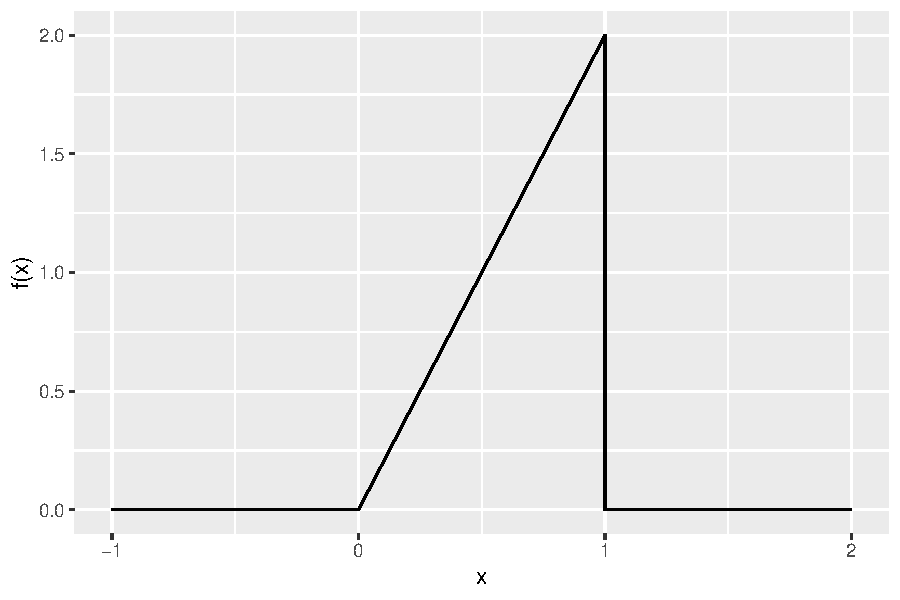
\includegraphics[height=.7\textheight]{figure/example-16-1-1}
    \end{center}
  \end{block}
\end{frame}



\begin{frame}
  \begin{block}{\examplectd}
    \begin{center}
      Cumulative Distribution Function

      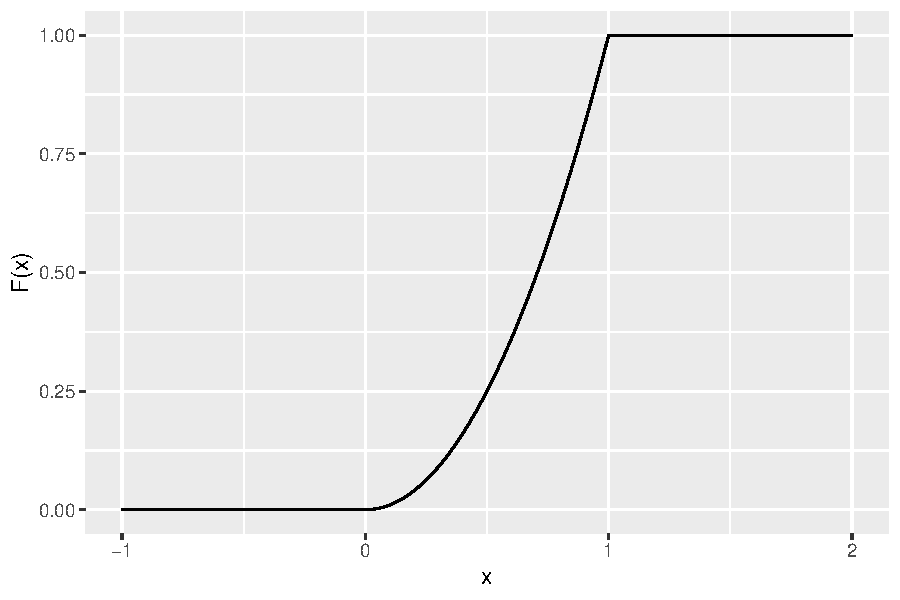
\includegraphics[height=.7\textheight]{figure/example-16-2-1}
    \end{center}
  \end{block}
\end{frame}



\begin{frame}<beamer:0>
  \begin{block}{\examplectd}
    \begin{tabular}{cc}
      $P(X < .5)$
      & $P(X \leq .5)$\\
      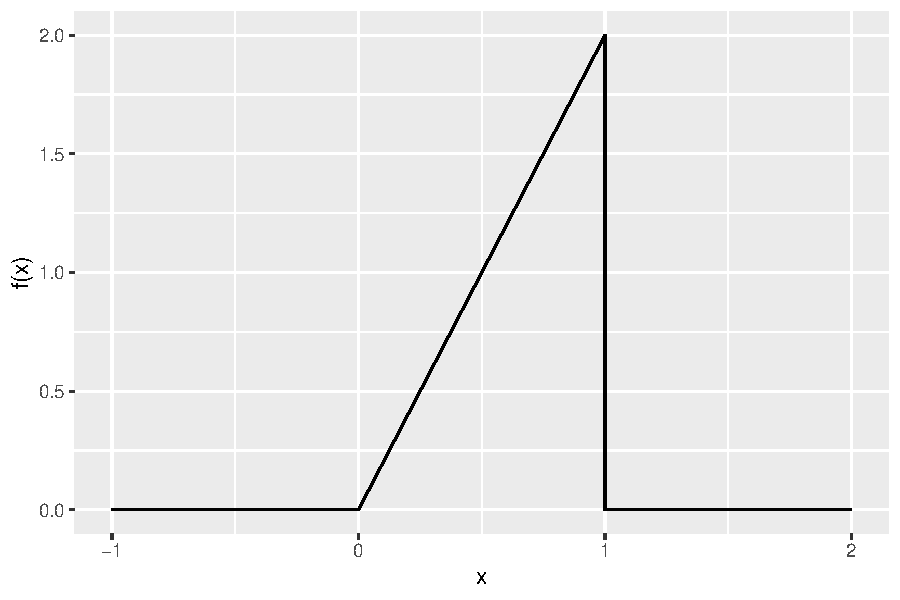
\includegraphics[height=.325\textheight]{figure/example-16-1-1}
      & 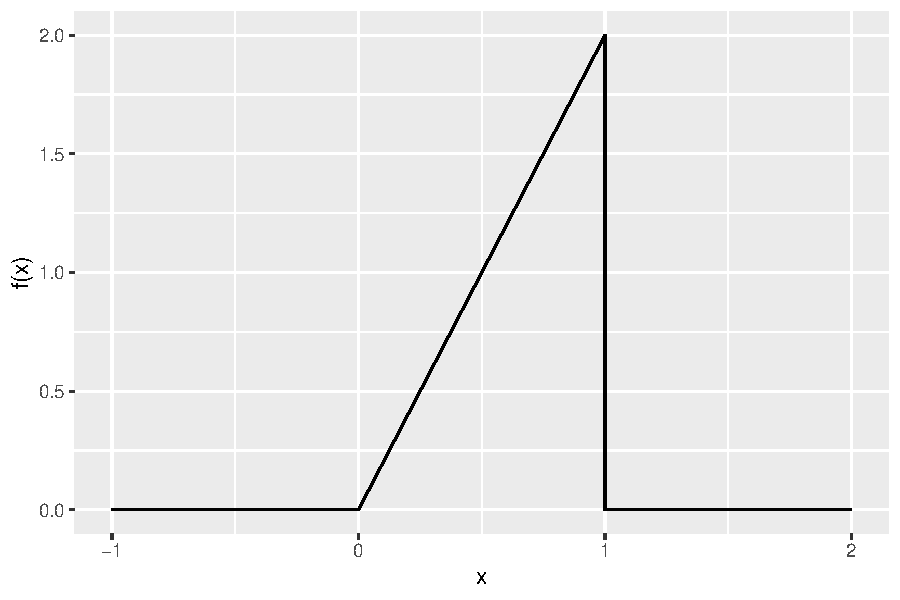
\includegraphics[height=.325\textheight]{figure/example-16-1-1}\\
      $P(.25 \leq X \leq .75)$
      & $P(X<.25 \mbox{ or } X >.75)$\\
      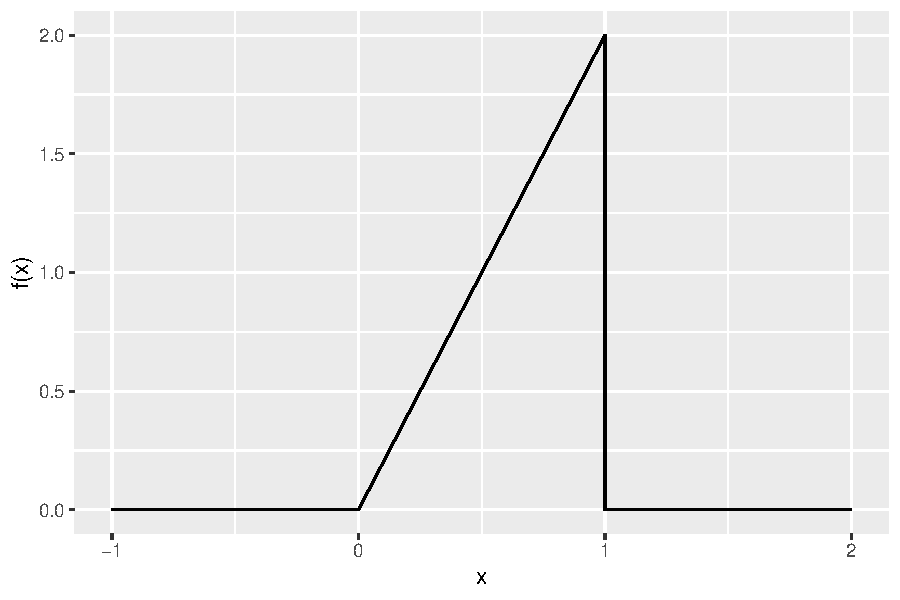
\includegraphics[height=.325\textheight]{figure/example-16-1-1}
      & 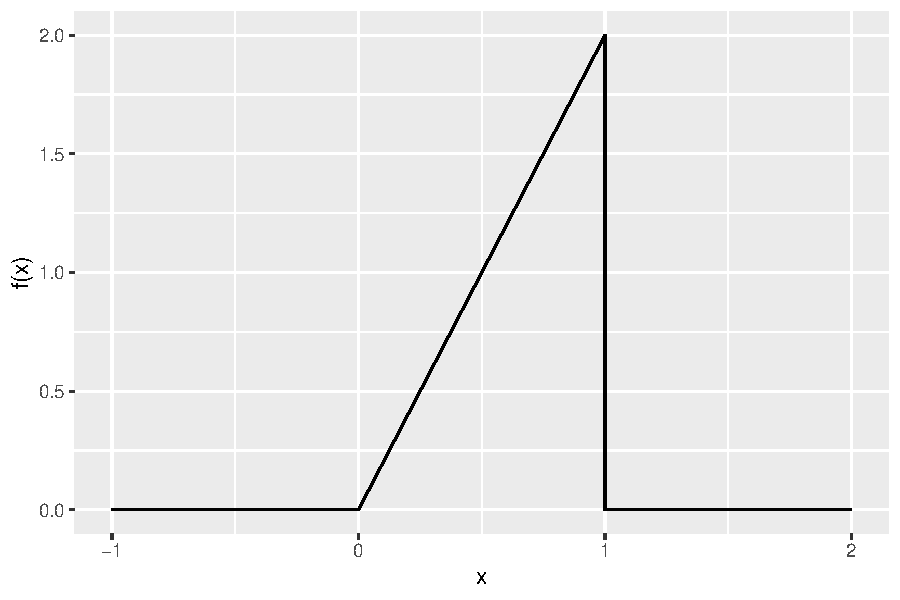
\includegraphics[height=.325\textheight]{figure/example-16-1-1}\\
    \end{tabular}
  \end{block}
\end{frame}

\begin{frame}<handout:0>
  \begin{block}{\examplectd}
    \begin{tabular}{cc}
      $P(X < .5)$
      & $P(X <=.5)$\\
      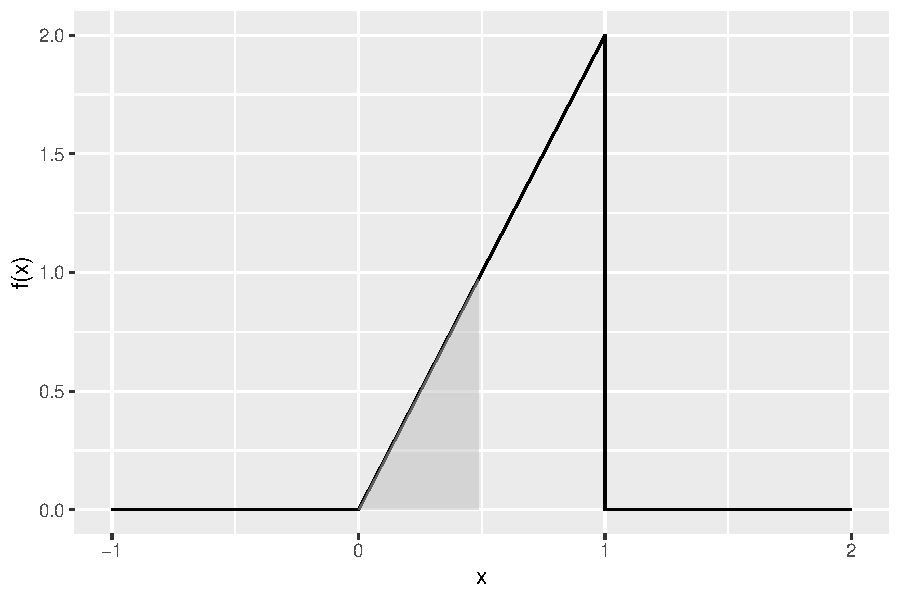
\includegraphics[height=.325\textheight]{figure/example-16-3-1}
      & 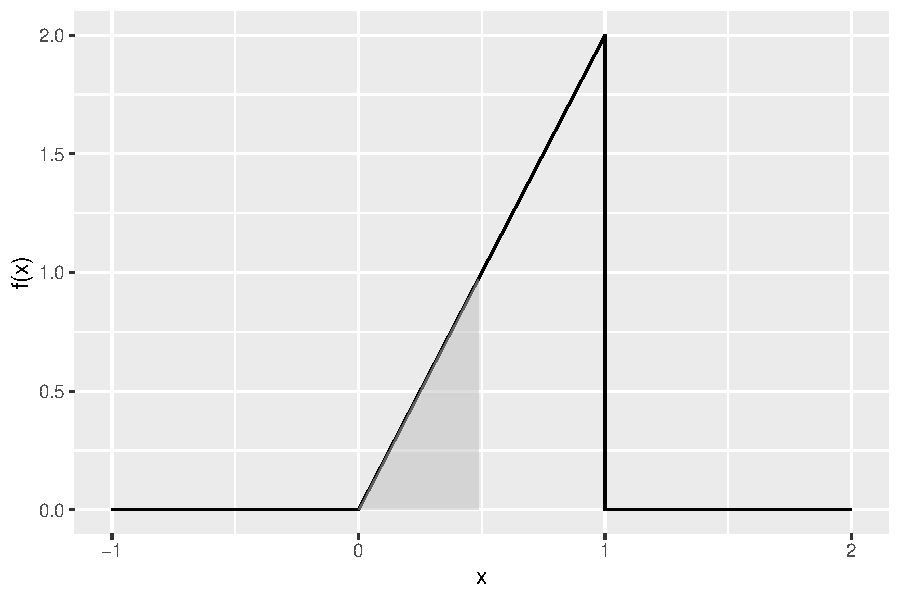
\includegraphics[height=.325\textheight]{figure/example-16-3-2}\\
      $P(.25 \leq X \leq .75)$
      & $P(X<.25 \mbox{ or } X >.75)$\\
      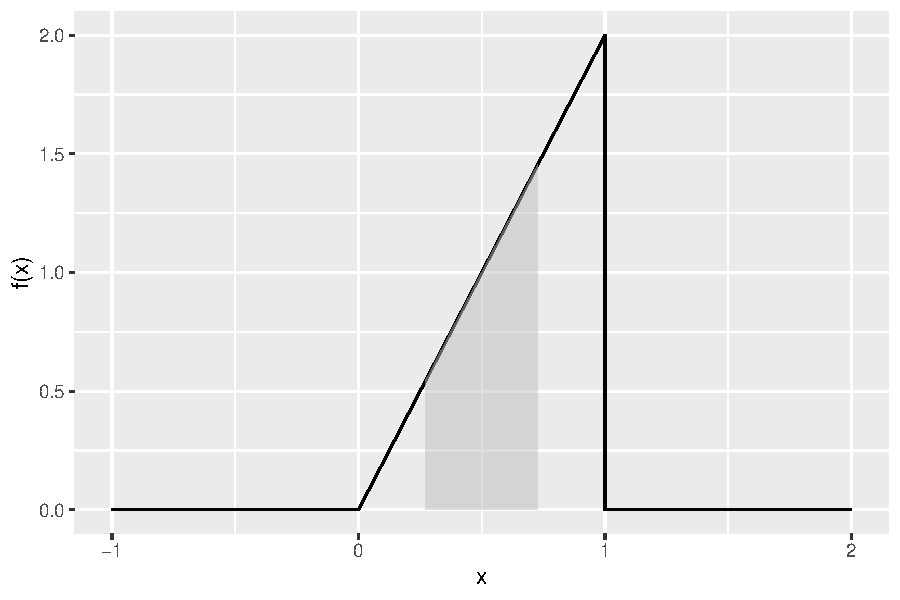
\includegraphics[height=.325\textheight]{figure/example-16-3-3}
      & 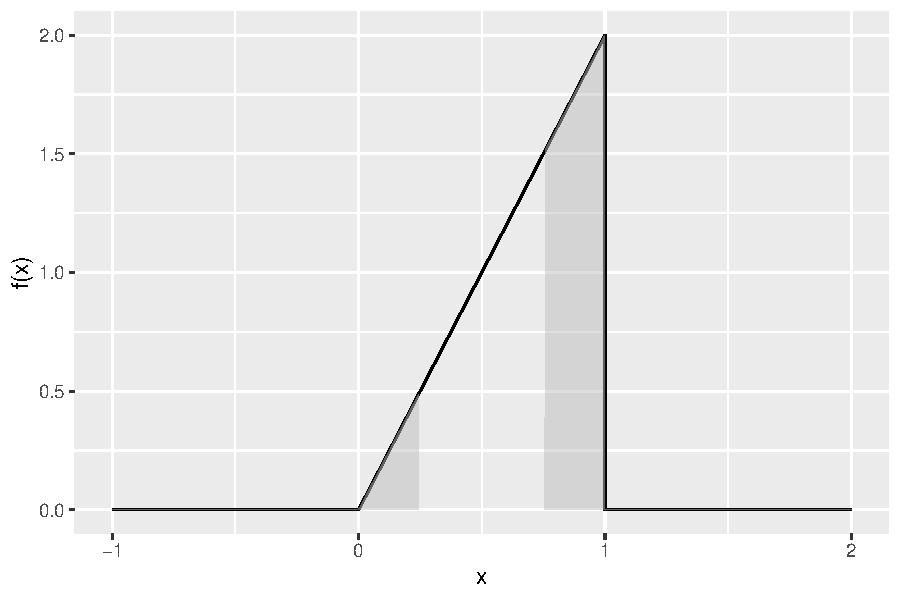
\includegraphics[height=.325\textheight]{figure/example-16-3-4}\\
    \end{tabular}
  \end{block}
\end{frame}

\begin{frame}

\begin{block}{Percentiles}

The $(100p)th$ percentile of a random variable $X$ is the value $\eta_p$ such that
$$
P(X \leq \eta_p)=F(\eta_p)=p.
$$

\medskip

Alternatively,
$$
\eta_p=F^{-1}(p).
$$
\end{block}

\end{frame}

\begin{frame}

\begin{block}{Median}

The median is the $50$th percentile, $\eta_{.5}$:
$$
P(X \leq \eta_{.5})=F(\eta_{.5})=.5.
$$

\medskip

Alternatively,
$$
\eta_{.5}=F^{-1}(.5).
$$
\end{block}

\end{frame}




\begin{frame}

\begin{block}{Probabilities and Quantiles}
    \begin{center}
      Cumulative Distribution Function
      
      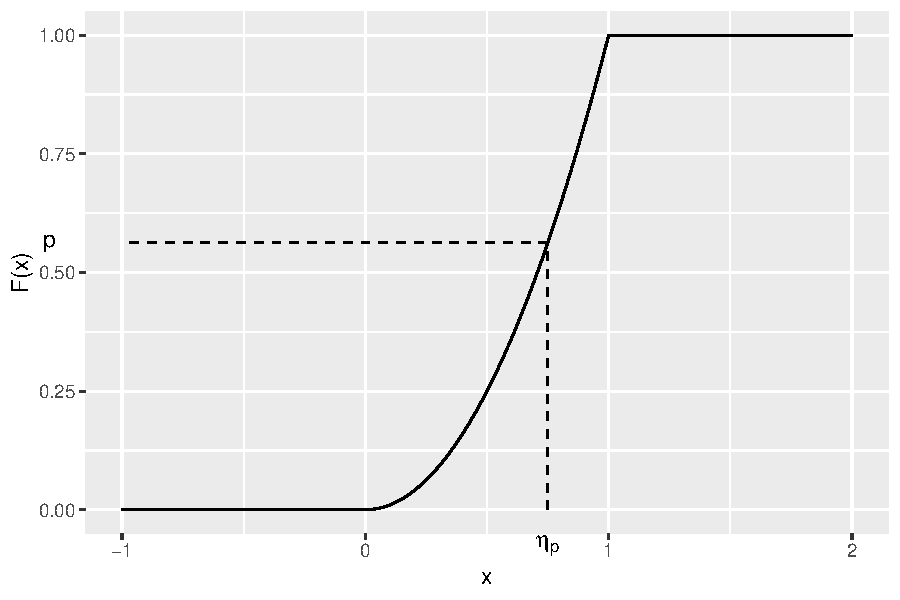
\includegraphics[height=.7\textheight]{figure/example-16-2b-1}
    \end{center}
  \end{block}

\end{frame}

\begin{frame}
  \begin{block}{\example}
    Let
    \[
      f(x)=
      \left\{
        \begin{array}{ll}
          0 & x \leq 0\\
          2x & 0 < x \leq 1\\
          0 & x > 1\\
        \end{array}
      \right.
    \]

    \begin{scriptsize}
      \begin{enumerate}[a)]
      \item Find the median of $X$.
      \item Find the $5$-th and $95$-th percentiles of $X$.
      \item What is the shortest interval, $(x_1,x_2)$, such that $P(x_1 < X <x_2)=.90?$
      %\item Find an alternative pdf that produces the same cdf.
      \end{enumerate}
    \end{scriptsize}
  \end{block}
\end{frame}

\begin{frame}<handout:0>
  \begin{center}
    \Huge{\textbf{Questions?}}
  \end{center}
\end{frame}

\begin{frame}
  \frametitle{\invisible{Hello}}

  \begin{center}
    \Large{\textbf{4.1 Continuous Random Variables}}

    \bigskip

    \large{\textbf{Some Comments}}
  \end{center}

  % \begin{center}
  %   
\includegraphics[height=.5\textheight]{roulette_wheel}
  % \end{center}

\end{frame}




\begin{frame}
  \begin{block}{Interpreting PDFs}
    \begin{enumerate}
    \item<1,2|handout:1-> Probability
      
      \only<2|handout:0>{
        For any interval, $\mathcal I$, with endpoints $a<b$
        \[
          P(X \in \mathcal I)=F(b)-F(a)=\int_a^b f(u)~du.
        \]
      }
    \item<1,3|handout:1-> Limit of histogram
    \item<1|handout:1-> Relative probability
    \end{enumerate}
  \end{block}
\end{frame}

\begin{frame}
  \begin{block}{Limit of Histogram}
  \begin{center}
    \begin{tabular}{cc}
      $n=10$
      & $n=100$\\
      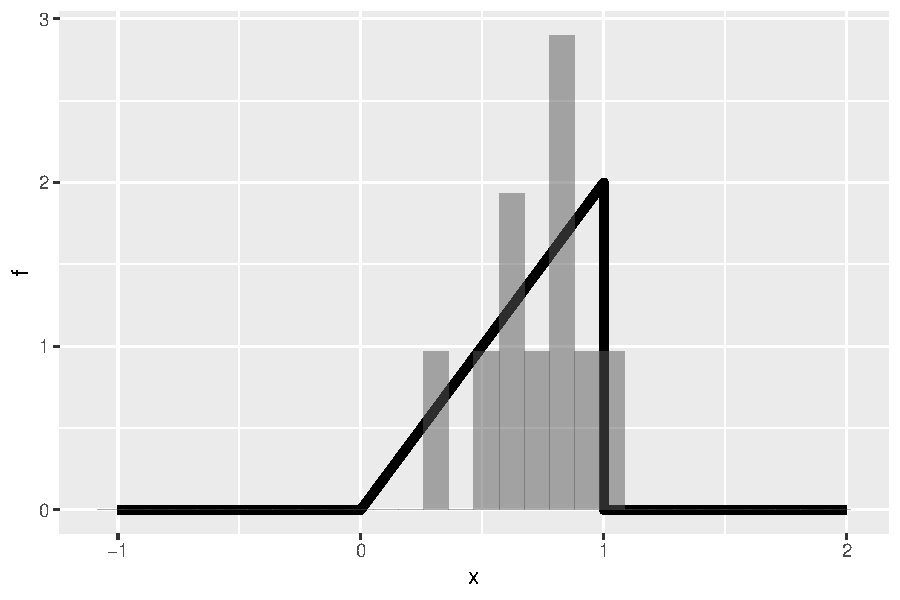
\includegraphics[height=.325\textheight]{figure/example-16-4-1}
      & 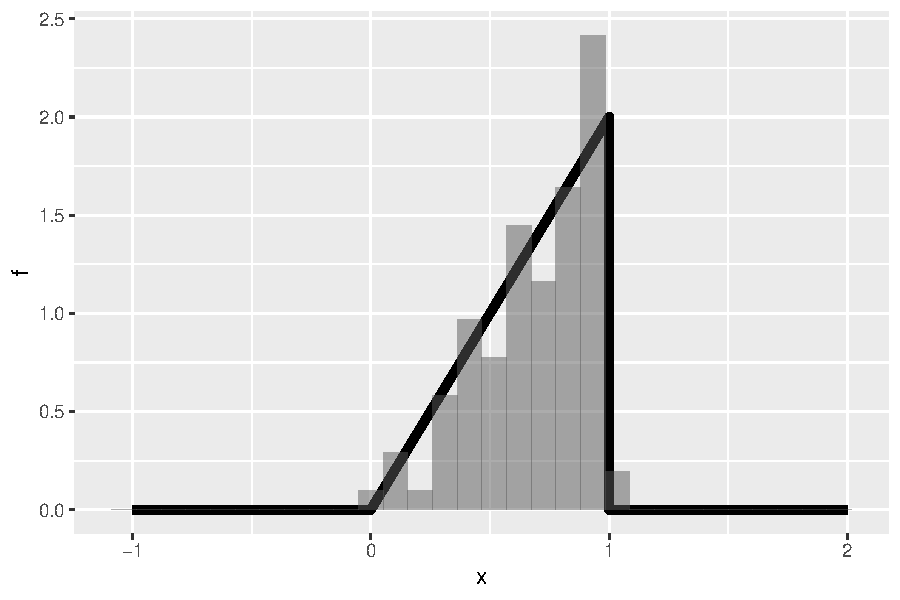
\includegraphics[height=.325\textheight]{figure/example-16-4-2}\\
      $n=1000$
      & $n=10000$\\
      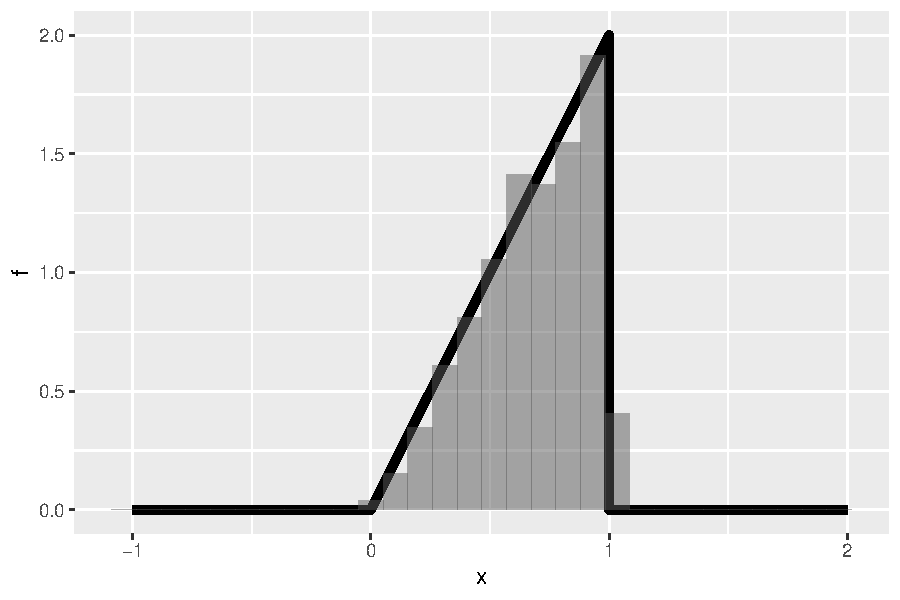
\includegraphics[height=.325\textheight]{figure/example-16-4-3}
      & 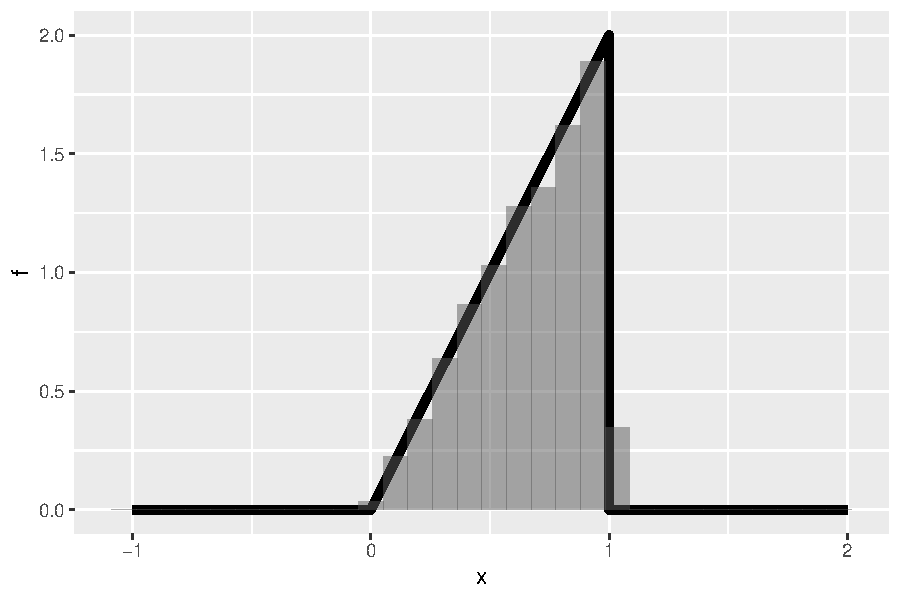
\includegraphics[height=.325\textheight]{figure/example-16-4-4}\\
    \end{tabular}
    \end{center}
  \end{block}
\end{frame}

\begin{frame}<handout:0>
  \begin{block}{Interpreting PDFs}
    \begin{enumerate}
    \item<beamer:0> Probability
      
    \item <beamer:0> Limit of histogram
      
    \item  Relative probability
      
        For any points $x_1,x_2 \in \Re$ at which $f(x)$ is continuous:
        \[
          \frac{P(X \in (x_1,x_1+\epsilon))}{P(X \in (x_2,x_2+\epsilon))}
          \approx
          \frac{\epsilon f(x_1)}{\epsilon f(x_2)}
          =\frac{f(x_1)}{f(x_2)}.
        \]
        
    \end{enumerate}
  \end{block}
\end{frame}



\begin{frame}
  \begin{block}{\examplectd}
    \begin{center}
      Probability Density Function

      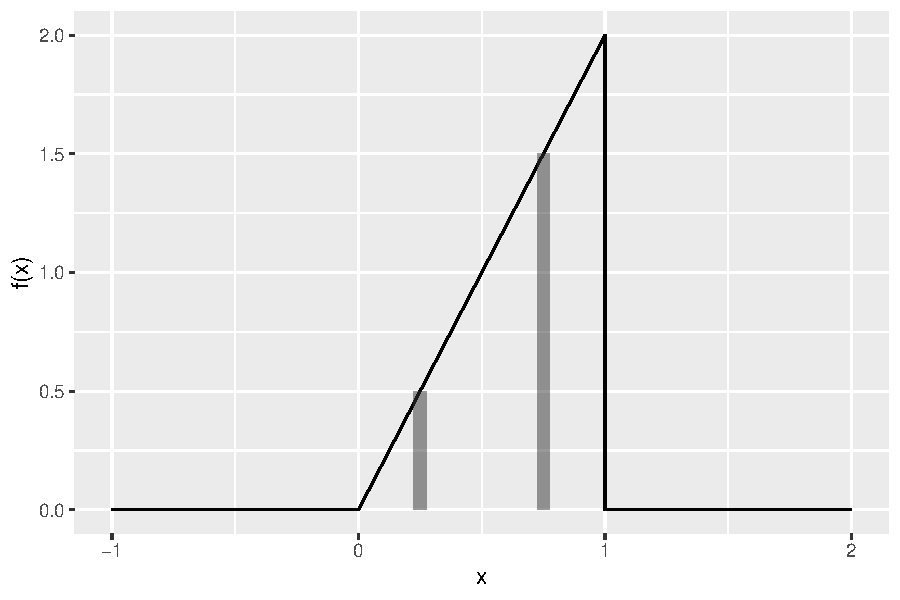
\includegraphics[height=.7\textheight]{figure/example-16-1b-1}
    \end{center}
  \end{block}
\end{frame}

% \begin{frame}<handout:0>
%   \begin{block}{Interpreting PDFs}
%     \begin{enumerate}
      
%     \item<beamer:0> Probability
      
%     \item <beamer:0> Limit of histogram
      
%     \item <beamer:0> Relative probability
        
%     \item Rate of change of cumulative probability
      
%       $f(x)$ measures the rate of change of $F(x)=P(X \leq x)$ at the point $x$
%     \end{enumerate}
%   \end{block}
% \end{frame}


%\begin{frame}
%  \begin{block}{Uniqueness of PDFs and CDFs}
%    The CDF of a continuous random variable \textbf{is unique}.
%
%    \bigskip
%
%    The PDF of a continuous random variable \textbf{is not unique}.
%  \end{block}
%\end{frame}


%\begin{frame}
%
%  \begin{block}{\example}
%    Consider the pdf
%    \[
%      f(x)=
%      \left\{
%        \begin{array}{ll}
%          0 & x \leq 0\\
%          2x & 0 < x \leq 1\\
%          0 & x > 1\\
%        \end{array}
%      \right.
%    \]
%     which has cdf
%     \[
%       F(x)=
%       \left\{
%         \begin{array}{ll}
%           0 & x \leq 0\\
%           x^2 & 0 < x < 1\\
%           1 & 1 \leq x
%         \end{array}
%       \right.
%     \]
%     Find another pdf that produces the same cdf.
% 
%   \end{block}
% \end{frame}

% \begin{frame}
%   \begin{block}{\examplectd}
%     Find a second function $g(x)$ such that:
%     \begin{enumerate}
%     \item $g(x)$ is a PDF
%     \item the CDF associated with $g(x)$ is the same as the CDF associated with $f(x)$
%     \end{enumerate}
%   \end{block}
% \end{frame}

\begin{frame}
  \begin{block}{Cumulative Distribution Functions}
    Any function $F(x)$ on $\mathbb R$ is a CDF if
    \begin{enumerate}
    \item $F(x)$ is non-decreasing
    \item $\lim_{x \searrow -\infty}F(x)=0$
    \item $\lim_{x \nearrow \infty}F(x)=1$
    \item $F(x)$ is continuous from the right
      \[
        \lim_{x \searrow c} F(x)=F(c)
      \]
      for all $c \in \Re$.
    \end{enumerate}

  \end{block}
\end{frame}

\begin{frame}
  \begin{block}{Discrete vs Continuous Random Variables}
    A random variable/probability distribution is continuous if $F(x)$ is continuous.

    \bigskip

    A random variable/probability distribution is discrete if $F(x)$ is a step function.

  \end{block}

\end{frame}

\begin{frame}<handout:0>
  \begin{center}
    \Huge{\textbf{Questions?}}
  \end{center}
\end{frame}

\begin{frame}

  \begin{block}{\exercise}
  
  Consider the distribution with cdf
  $$
  F(X)=
  \left\{
  \begin{array}{ll}
  0 & x < 0\\
  \log_{10}(x + 1) & 0 \leq x < 9\\
  1 & 9 \leq x
  \end{array}
  \right.
  $$
  
  \begin{enumerate}[a)]
  \item Plot $F(x)$.
  \item Compute the pdf, $f(x)$.
  \item Plot $f(x)$.
  \item Compute the following probabilities:
  \begin{enumerate}[i.]
  \item $(X \leq \sqrt{10}\textcolor{red}{-1})$
  \item $P(X < \sqrt{10} \textcolor{red}{-1})$
  \item $P(X = \sqrt{10}\textcolor{red}{-1})$
  \item $P(X > \sqrt{10}\textcolor{red}{-1})$
  \item $P(X \geq \sqrt{10}\textcolor{red}{-1})$
  \end{enumerate}
  \end{enumerate}
  \end{block}
\end{frame}

\end{document}
